\documentclass[11pt,a4paper,oneside]{report}             % Single-side
%\documentclass[11pt,a4paper,twoside,openright]{report}  % Duplex

%\PassOptionsToPackage{chapternumber=Huordinal}{magyar.ldf}
\usepackage{t1enc}
\usepackage[latin2]{inputenc}
\usepackage[magyar, german, english]{babel}
\usepackage{mathtools}
\usepackage{amssymb}
\usepackage{siunitx}
\usepackage{enumerate}
\usepackage{pgfplots, pgfplotstable}
\usepackage[thmmarks]{ntheorem}
\usepackage{graphics}
\usepackage{multirow}
\usepackage{graphicx,floatpag,fancyhdr}
\usepackage{epsfig}
\usepackage{listings}
\usepackage{color}
\usepackage{lastpage}
\usepackage{anysize}
\usepackage{sectsty}
\usepackage{setspace}  % Ettol a tablazatok, abrak, labjegyzetek maradnak 1-es sorkozzel!
\usepackage[hang]{caption} 
\usepackage{subcaption}
\usepackage{hyperref}
\usepackage{afterpage}
\usepackage{booktabs}
% Own inclusions
\usepackage{titlesec}
\usepackage{relsize}
\usepackage{anyfontsize}
\usepackage{pdfpages}
\usepackage{makeidx}
%\usepackage{adjustbox}
\usepackage[export]{adjustbox}
\usepackage{enumitem}
\usepackage[inkscapeopt= -D -z]{svg}

%--------------------------------------------------------------------------------------
% SVG package setup
%--------------------------------------------------------------------------------------
\setsvg{inkscape={"C:/Program Files/Inkscape/inkscape" -D -z}}

%--------------------------------------------------------------------------------------
% Path setups: figures, svgs, tables, charts
%--------------------------------------------------------------------------------------
\svgpath{{"C:/Users/{"Barancsuk_Lilla"}/Documents/{"current_semester"}/Dipterv_repo/{"Latex_document"}/figures/"}}
\graphicspath{{figures/}{figures/for_timelines/}{figures/for_frames/}{figures/GT/}{figures/calcorr/fovam/}{figures/calcorr/ibike/}{figures/calcorr/}{figures/calcorr/uncalib/}}

\newcommand{\tablepath}{tables/}

\makeatletter
\newcommand{\includetable}[1]{%
	\@ifundefined{tablepath}{%
		\InputIfFileExists{#1}{}{}%
	}{%
		\InputIfFileExists{\tablepath/#1}{}{\InputIfFileExists{#1}{}{}}%
	}
}
\makeatother 

\newcommand{\chartpath}{charts/}

\makeatletter
\newcommand{\includechart}[1]{%
	\@ifundefined{chartpath}{%
		\InputIfFileExists{#1}{}{}%
	}{%
		\InputIfFileExists{\chartpath/#1}{}{\InputIfFileExists{#1}{}{}}%
	}
}
\makeatother 

%--------------------------------------------------------------------------------------
% Main variables
%--------------------------------------------------------------------------------------
\newcommand{\vikszerzo}{Lilla \textsc{Barancsuk}}
\newcommand{\vikkonzulens}{Krist�f \textsc{Csorba}, PhD}
\newcommand{\vikcim}{Development and integration of camera based traffic monitoring system}
\newcommand{\viktanszek}{Department of Automation and Applied Informatics}
\newcommand{\vikdoktipus}{Masters thesis}
\newcommand{\vikdepartmentr}{Barancsuk Lilla}

%--------------------------------------------------------------------------------------
% Page layout setup
%--------------------------------------------------------------------------------------
% we need to redefine the pagestyle plain
% another possibility is to use the body of this command without \fancypagestyle
% and use \pagestyle{fancy} but in that case the special pages
% (like the ToC, the References, and the Chapter pages)remain in plane style

\pagestyle{plain}
%\setlength{\parindent}{0pt} % �ttekinthet�bb, angol nyelv� dokumentumokban jellemz�
%\setlength{\parskip}{8pt plus 3pt minus 3pt} % �ttekinthet�bb, angol nyelv� dokumentumokban jellemz�
\setlength{\parindent}{12pt} % magyar nyelv� dokumentumokban jellemz�
\setlength{\parskip}{0pt}    % magyar nyelv� dokumentumokban jellemz�

\marginsize{35mm}{25mm}{15mm}{15mm} % anysize package
\setcounter{secnumdepth}{0}
\sectionfont{\large\upshape\bfseries}
\setcounter{secnumdepth}{2}
\singlespacing
\frenchspacing

% This defines the fancy page style to be similar to plain
\pagestyle{fancy}
\fancyhf{}% Clear header/footer
\fancyfoot[C]{\thepage}
\renewcommand{\headrulewidth}{0pt}% Remove header rule

% Page style plainlower is similar to plain, but lowers page number by 6 lines of text
\fancypagestyle{plainlower}{
	\fancyhf{}% Clear header/footer
	\fancyfoot[C]{\raisebox{-6\baselineskip}{\thepage}}
	\renewcommand{\headrulewidth}{0pt}% Remove header rule
}

%--------------------------------------------------------------------------------------
%	Setup hyperref package
%--------------------------------------------------------------------------------------
\hypersetup{
    %bookmarks=true,            % show bookmarks bar?
    unicode=false,             % non-Latin characters in Acrobat�s bookmarks
    pdftitle={\vikcim},        % title
    pdfauthor={\vikszerzo},    % author
    pdfsubject={\vikdoktipus}, % subject of the document
    pdfcreator={\vikszerzo},   % creator of the document
    pdfproducer={Producer},    % producer of the document
    pdfkeywords={keywords},    % list of keywords
    pdfnewwindow=true,         % links in new window
    colorlinks=true,           % false: boxed links; true: colored links
    linkcolor=black,           % color of internal links
    citecolor=black,           % color of links to bibliography
    filecolor=black,           % color of file links
    urlcolor=black             % color of external links
}

%--------------------------------------------------------------------------------------
% Set up listings
%--------------------------------------------------------------------------------------
\lstset{
	basicstyle=\scriptsize\ttfamily, % print whole listing small
	keywordstyle=\color{black}\bfseries\underbar, % underlined bold black keywords
	identifierstyle=, 					% nothing happens
	commentstyle=\color{white}, % white comments
	stringstyle=\scriptsize\sffamily, 			% typewriter type for strings
	showstringspaces=false,     % no special string spaces
	aboveskip=3pt,
	belowskip=3pt,
	columns=fixed,
	backgroundcolor=\color{lightgray},
} 		
\def\lstlistingname{code-listing}	

%--------------------------------------------------------------------------------------
%	Some new commands and declarations
%--------------------------------------------------------------------------------------
\newcommand{\code}[1]{{\upshape\ttfamily\scriptsize\indent #1}}
\newcommand{\reg}{\textsuperscript{\textcircled{\textsc r}}}
% define references
\newcommand{\figref}[1]{\ref{fig:#1}.}
\renewcommand{\eqref}[1]{(\ref{eq:#1})}
\newcommand{\listref}[1]{\ref{listing:#1}.}
\newcommand{\sectref}[1]{\ref{sect:#1}}
\newcommand{\tabref}[1]{\ref{tab:#1}.}
\newcommand{\hsp}{\hspace{0pt}}

%--------------------------------------------------------------------------------------
% Math operators
%--------------------------------------------------------------------------------------
\DeclareMathOperator*{\argmax}{arg\,max}
%\DeclareMathOperator*[1]{\floor}{arg\,max}
\DeclareMathOperator{\sign}{sgn}
\DeclareMathOperator{\rot}{rot}
\DeclareMathOperator{\avg}{avg}
\DeclareMathOperator{\avgt}{\underset{\textit{t}}{avg}}
%Math mode set\part{title}
%\everymath{\displaystyle}

%--------------------------------------------------------------------------------------
%Color declarations
%--------------------------------------------------------------------------------------
\definecolor{lightgray}{rgb}{0.95,0.95,0.95}
\definecolor{indigo}{RGB}{47, 27, 60}
\definecolor{darkviolet}{RGB}{62, 44, 102}
\definecolor{lightviolet}{RGB}{96, 92, 153}
\definecolor{taupe}{RGB}{176, 158, 141}
\definecolor{lighttaupe}{RGB}{216, 208, 197}
\definecolor{camel}{RGB}{232, 208, 174}

%--------------------------------------------------------------------------------------
%Chart color cycle
%--------------------------------------------------------------------------------------
\pgfplotscreateplotcyclelist{violets}{
	{fill=indigo!60!white, draw=indigo},
	{fill=taupe!60!white, draw=taupe},
	{fill=darkviolet!60!white, draw=darkviolet},
	{fill=camel!60!white, draw=camel},
	{fill=lightviolet!60!white, draw=lightviolet},
}


%--------------------------------------------------------------------------------------
%Chart setup
%--------------------------------------------------------------------------------------
\newcommand{\placelegend}{legend style={at={(1.2,1)}, anchor=north, legend columns=1},}
\newcommand{\custombarwidth}{0.13cm}
%--------------------------------------------------------------------------------------
% Includes
%--------------------------------------------------------------------------------------
\author{\vikszerzo}
\title{\viktitle}
\includeonly{
	guideline,%
	project,%
	titlepage,%
	declaration,%
	abstract,%
	introduction,%
	chapter1,%
	%chapter2,%
	chapter3,%
	chapter4,%
	chapter5,%
	conclusions,%
	acknowledgement,%
	appendices,%
}

%--------------------------------------------------------------------------------------
%	Setup captions
%--------------------------------------------------------------------------------------
\captionsetup[figure]{
%labelsep=none,
%font={footnotesize,it},
%justification=justified,
width=.75\textwidth,
aboveskip=10pt}

\renewcommand{\captionlabelfont}{\small\bf}
\renewcommand{\captionfont}{\footnotesize\it}

%---------------
% makeindex
%---------------
\makeindex
%--------------------------------------------------------------------------------------
% Table of contents and the main text
%--------------------------------------------------------------------------------------
\begin{document}

%-------------------------------------------------------------------
%	Chapter header format with HUGE numbering <3 <3 <3 (Because it's pretty)
%-------------------------------------------------------------------
\titleformat{\chapter}[display]{\flushright\fontseries{b}\fontsize{120}{120}\selectfont}{\fontseries{b}\fontsize{180}{4}\selectfont\thechapter\hsp}{0pt}{\Huge\bfseries}[]

\singlespacing
\pagenumbering{arabic}
\onehalfspacing
\includepdf[pages={1}]{../Kameras-forgalomszamlalo-rendszer-fejlesztese-Feladatkiiras-2.pdf}
\include{titlepage}
\tableofcontents\vfill
\include{declaration}
%----------------------------------------------------------------------------
% Abstract in hungarian
%----------------------------------------------------------------------------
\chapter*{Kivonat}\addcontentsline{toc}{chapter}{Kivonat}

Amellett, hogy a k�zutak forgalmi adatainak nyilv�ntart�sa az �nkorm�nyzatok k�telez� feladata, a forgalomsz�ml�l�s sokf�le �rt�kes inform�ci�t szolg�ltat. Seg�ts�g�vel megbecs�lhet� az adott �tszakasz k�rosanyag-kibocs�t�sa �s terhelts�ge, amivel hozz�j�rul a megl�v� �th�l�zat �zemeltet�s�hez, beruh�z�sok tervez�s�hez. A real-time forgalomsz�ml�l� rendszerek pedig alkalmasak forgalmi dug�k detekt�l�s�ra, megel�z�s�re is.

Napjainkban a k�zi forgalomsz�ml�l�st egyre ink�bb felv�ltj�k az automatiz�lt m�dszerek. 
A radaros �s az �tba �p�thet� (indukt�v hurkos) rendszerek mellett a videofelv�tel alapj�n t�rt�n� sz�ml�l�s �rvend a legnagyobb n�pszer�s�gnek. 
A korl�tozott er�forr�s�, be�gyazott k�rnyezetben azonban tov�bbra is kih�v�st jelent a k�pfeldolgoz�son alapul� sz�ml�l�s val�sidej� megval�s�t�sa. 
Az elterjedt, nagy sz�m�t�sig�ny� h�tt�r-elt�vol�t�st �s feature-pont k�vet�st haszn�l� megold�sok sokszor nem �rik el a k�v�nt pontoss�got vagy sebess�get.

Dolgozatomban egy, a forgalomt�meg becsl�s�re alkalmas rendszert mutatok be, amely az utat fel�lr�l r�gz�t� kamera k�p�t dolgozza fel. 
C�lom egy olyan l�mpatestbe �p�thet� intelligens szenzor megalkot�sa volt, amely adott korl�tos er�forr�s� hardveren is k�pes val�s id�ben m�k�dni, az elhalad� j�rm�vek sz�m�t, t�pus�t adott pontoss�ggal meg�llap�tani, valamint megbecs�li sebess�g�ket �s k�vet�si t�vols�gukat.

Dolgozatomban r�szletesen bemutatom a rendszer magj�t alkot� szoftver m�k�d�s�t �s fel�p�t�s�t, valamint a vide�k�pek feldolgoz�s�nak folyamat�t, melynek alapja t�bbf�le, hat�kony vide�feldolgoz�si m�dszer �sszekapcsol�sa: h�tt�r-elt�vol�t�s, tripwire-alap� sz�ml�l�s, ill. kis sz�m�t�sig�ny� adatgy�jt�s �s oszt�lyoz�s kombin�l�sa, ezek el�nyeinek egyes�t�se.
Kit�rek a rendszert kieg�sz�t�, a val�s forgalomban val� m�k�d�st lehet�v� tev� szoftver- �s hardverk�rnyezetre, a t�volr�l t�rt�n� kalibr�ci�t �s tesztel�st megval�s�t� alkalmaz�sra �s a rendszer konfigur�ci�j�nak menet�re.
R�szletezem az alkalmaz�s pontoss�g- �s se\-bes\-s�g\-tesz\-te\-l�\-s�\-nek mik�ntj�t, a tesztek eredm�ny�t, valamint a tov�bbfejl�d�s lehets�ges �tjait is.
\vfill

%----------------------------------------------------------------------------
% Abstract in english
%----------------------------------------------------------------------------
\chapter*{Abstract}\addcontentsline{toc}{chapter}{Abstract}

The registration of traffic data of public roads is not only a compulsory task of local governments, but the traffic count provides valuable information of various kinds. It can be used to estimate the pollution emission and load of a road, which contributes to the operation of the current facilities and to the appropriate planning of new investments. Moreover, real-time traffic monitoring systems are able to detect and even to avoid traffic jams, too.

Nowadays, manual surveillance are more and more being replaced by automatized methods. Besides the radar-based systems and inductive loop detectors installed in the road, the video-based traffic detection is among the most popular methods. However, its real-time implementation, by means of image processing, is still challenging in resource-limited embedded systems. The popular algorithms of background subtraction and feature point tracking are usually associated with a computational cost being too high to meet the accuracy and speed requirements.

In this work, I introduce a system for traffic flow estimation, based on the processing of a video stream of a camera installed above the road. My goal was to device an intelligent sensor that can be installed within a street-lighting lamp, which operates in real-time on the given resource-limited hardware. It is able to determine the number and type of the vehicles passing by with an acceptable accuracy, and also to estimate their speed and following distance.

The operation and architecture of the core software and the video processing task is presented in detail in this work. The main idea is the combination of various efficient video processing methods: background subtraction, tripwire-based counting, data mining and classification algorithms of low computational cost, respectively. The benefits of each algorithm is exploited via their appropriately combined use.
The supplementary software and hardware elements, which facilitate the remote calibration, testing, and the configuration process are discussed.
Moreover the accuracy and speed testing process and the results are presented along with possible ways of further improvement.
\vfill


%----------------------------------------------------------------------------
\chapter*{Introduction}\addcontentsline{toc}{chapter}{Introduction}
%----------------------------------------------------------------------------
\section{Traffic load estimation}
%----------------------------------------------------------------------------
In recent years, there has been an increased scope for the automatic analysis of urban traffic activity\cite{Buch2011}.
This case is due to the increasing number of vehicles, the need for better understanding traffic dynamics for investment purposes, and also the accessibility of various sensors.
Formerly traffic estimation was performed by operators, by the means of on-the-spot observation or video analysis.
Automating these processes, the main concept of traffic analysis is to aid or fully avoid human operators.

The information obtained by traffic monitoring systems are widely used to regulate traffic flow and contribute to administrative decisions about transportation infrastructure development, maintenance and investments \cite{MagyarKozut}.
In addition to the detection and classification of road users, which is an elementary task, several other monitoring objectives can be supported. 
Typical traffic data such as flow, density, and average speed can be extracted.
Some systems also recognize various situations including traffic violations or accidents (e.g., cars, motorbikes, and pedestrians).
Other real-time applications notify users about congestions, roadworks and accidents, or control traffic lights in order to influence traffic flow intensity in one direction \cite{AzoSensor, Thiruverahan2015, Ghazal2016}.
It is also possible to estimate environmental measures such as greenhouse gases, pollutant emissions, and fuel consumption in real time using high-resolution video traffic data combined with instantaneous emission models\cite{Morris2012a}. 
In the long term surveillance systems will be integral parts of the smart city infrastructure, modelling, identifying and influencing these city's traffic dynamics\cite{enLight}.

\subsection{Traffic monitoring techniques}
Nowadays a variety of sensing modalities is available for on-road vehicle detection.

Inductive loop systems installed in the road are considered the most reliable traffic classification and detection method available, since larger metal objects can be accurately detected this way. 
On the other hand, the installation and maintenance is time-consuming and difficult, and slow or temporarily stopped vehicles cannot be detected\cite{Diamond, Zhang2016}.

Other active detection methods, including radar \cite{DeepBlue}, infrared\cite{Swarco, Hussain1995, Ghazal2016} and laser\cite{SICK, Gallego2009} sensors, are also popular owing to their robustness, although a complex machinery needs to be deployed.

Weight-based classification and speed detection is also possible using a piezoelectric sensor\cite{Te, Rivas2017}.

Video cameras have been installed for a long time for traffic monitoring purposes, because they provide a rich information source for human understanding with a relatively low cost of deployment\cite{Tian2011, Buch2011, VideoSurveillance, LaSemaforica}.
Nowadays cameras became even cheaper, smaller, and of higher quality than ever before, and vision-based surveillance is becoming the most popular form of vehicle detection.
In contradistinction to active sensors, cameras provide a wide field of view, allowing for detection across multiple lanes. 
Vision also integrates well with active sensor suites\cite{Garcia2012}.
The drawbacks to vision-based vehicle detection include sensitivity to light and weather conditions and increased computational cost\cite{Shivaraman2013}.

Multi-modal suites use sensor fusion to combine the data that results from the approaches outlined above\cite{Swarco}.

\subsubsection{Real-time vision sensors}
Although most vision sensor networks use a digital backend system where the captured data is transferred, and computation and storage takes place, since computing power has dramatically increased in the recent years, a new generation of visual surveillance systems has emerged.
These embedded sensors are capable of on-board high-level video processing with limited resources for computation, memory and power \cite{Bramberger2004}.
These platforms have the ability to reliably detect and track on-road vehicles in real time, since they utilize the new image-processing paradigms and advanced hardware: parallelization, multi-core processing and graphical processing units (GPUs)\cite{Sivaraman2013}.
Although the embedded platforms can provide sufficient computing performance, efficiently developing and porting software for these platforms is still a difficult and tedious task\cite{Bramberger2004}.
In this thesis an efficient traffic estimation method for embedded hardware is proposed, which can operate in real time for extended periods.
The implementation and realization details are discussed in the following chapters.

\subsection{Some results in video-based traffic monitoring}
In this section approaches in video-based on-road traffic monitoring are discussed, in particular with regard to techniques used in monocular vision.

Even though very diverse solutions has been suggested in the literature for vision-based surveillance problems, these methods are similar in the fact that they utilize the high information-content of the video stream, whilst the useless data are being identified and omitted for speed purposes.

Most vehicle counting methods are composed of three levels of perception depending upon each other: detection, tracking and behaviour understanding.
The two upper levels use information extracted from the lower ones, since vehicles are continuously detected across several frames for tracking purposes, and behaviour understanding relies strongly on the trajectory of the object.

At the first level, the goal is to tell vehicles apart from the background using distinctive features: appearance or motion.

On of the two main approaches is appearance-based selection, wherein basic image characteristics such as colour\cite{Chang2005}, edges\cite{Blanc2007}, symmetry\cite{Aytekin2010}, HOG\cite{TehraniNiknejad2012}, Haar-like\cite{Sivaraman2012}, Gabor\cite{Zhang2006}, SIFT\cite{Zhang2011} or SURF\cite{Lin2012} features are used to identify vehicles.
In recent years, there has been a transition from simpler image features like edges and symmetry to general and robust feature sets\cite{Sivaraman2012}.
These detection methods are both applicable for moving and stationary objects or cameras, but requires prior information about foreground object appearances.

These extracted features along with others are widely used for vehicle classification.
Most common distinctive attributes are heigh and length\cite{Huang2004}, linearity feature -- meaning the roughness of the vehicle contour\cite{Zhang2008} --, convex hull of the silhouette\cite{Buch2010} and distance between contour points\cite{Lou2005}.
Well-known descriptors like SIFT\cite{Zhang2011}, SURF\cite{Lin2012}, HOG\cite{Niknejad2012a} and a handful of others are also popular.
Automatic license plate recognition, which is also extensively used, relies on these features\cite{Luvizon2016}. 

Classifiers can be broadly split into two categories: the less popular discriminative classifiers, that learn the underlying distribution of a given class; and generative ones relying upon hard decision boundaries between classes\cite{Sivaraman2012}.
Discriminative methods include artificial neural network classifiers\cite{Xia2006}, support vector machines\cite{Cornelis2008}, k-nearest neighbour (kNN) classifier\cite{Morris2006}, and AdaBoost\cite{Khammari2005}.
Popular generative classifiers are hidden Markov models\cite{Jazayeri2011}, probabilistically weighted vote\cite{Lin2012}, and hidden random field\cite{Zhang2011}.

Motion-based vehicle detection has been less common than appearance-based methods.
The core idea is to separate moving foreground from motionless background.
This approach relies on background subtraction: the static scene is estimated with various models and moving object are separated accordingly.
Several filters have been proposed for background subtraction, including frame differencing\cite{Park2007}, averaging\cite{Kanhere2008}, graph cuts\cite{Woodford2009}, as well as more sophisticated background models, such as Single Gaussian\cite{Kumar2003}, mode estimation\cite{Zheng2006}, Kalman-filter\cite{Messelodi2005} or wavelets\cite{Gao2009}. 

One of the most common subtraction techniques is Gaussian Mixture Modelling(GMM)\cite{Niknejad2012, Wang2009,Zhang2016a}, wherein each pixel is temporally modelled as a mixture of two or more Gaussians and is updated online\cite{Stauffer1999,Stauffer2000}.
GMM is considered one of the best parametric background models that are widely used, owing to its robustness and effectiveness over different scenes\cite{Zhang2016}.
Although most subtraction techniques assume a fixed scene, GMM can deal with both stationery backgrounds and repetitive changes in light.
The implementation in \cite{Kaewtrakulpong2001} is available in the OpenCV library and is commonly used in research\cite{OpenCVMog2}.

One level up dynamic parameters are measured and the position of road-users is approximated using various tracking algorithms. 
The main purposes of following vehicles across frames is to estimate  motion, predict vehicle positions, and enforce temporal coherence to omit false positives in counting.
Tracking algorithms range from simplest -- like geometric constraints\cite{Rabe2007}, optical flow\cite{Bhaskar2015}, template matching\cite{Liu2007}, feature-based tracking\cite{Haselhoff2009} -- to most complex, including particle filtering\cite{Danescu2011}, Kalman-filter\cite{Bresson2015}, spatial–temporal Markov random field (S-T MRF)\cite{Zhu2005}, graph correspondence\cite{Lai2010} and event cones\cite{Andrienko2015} along with others. 

The highest level of semantic interpretation lies in characterizing the behaviour of vehicles on the road\cite{Sivaraman2013}.
An aggregate of spatio-temporal features is used to learn, model, classify, and predict the behaviour and goals of other vehicles on the road.
Certain studies categorize observed vehicle behaviour as normal or critical\cite{Cherng2009}, others identify specific maneuvers, like lane changing or turning\cite{Garcia2012}, some works try to forecast vehicle trajectory using trajectory-based predictors\cite{Hermes2009}, others focus on incident detection\cite{Kamijo2004}.
Maneuver-classification methods include hidden Markov model\cite{Sivaraman2011}, Bayesian networks\cite{Kasper2012} as well as Gaussian mixture modeling\cite{Wiest2012}.

Handling extreme weather or light conditions is always challenging for visual sensors, therefore a series of different solutions has been proposed to be able to process scenes with rain\cite{Yu2015,Barnum2010}, thick fog\cite{Zhou2014a,Tarel2009}, night-time\cite{Bi2009, Robert2009} or heavy shadows\cite{Kamkar2016, Miller2015}.

\subsubsection{Counting vehicles with time-spatial images}
Many traditional methods fail in real-time, embedded environments for traffic counting purposes, due to their high computational complexity.
Hence one of the challenges of real-time traffic monitoring is to decrease the aforementioned computation time by minimizing the information processed by filtering the image domain.

The selection of relevant information often relies on a priori knowledge of the scene, including direction of traffic flow and assumed trajectory of bypassing vehicles.
Many of these selection techniques restrict the calculation to an interested region in the traffic scene, e.g. virtual loops\cite{Tursun2013a, He2008} or detection regions\cite{Miller2015s, Engel2016} placed in the way of vehicles.

One of the most cost-effective, image-domain reducing techniques is based on virtual detection lines (VDLs) and time-spatial images (TSIs).
A virtual detection line is a one-pixel wide straight line placed perpendicular or parallel to the vehicle trajectory, whilst a time-spatial image can be considered itself as an image, where the vertical dimension corresponds to the VDL in the original frame, and the horizontal one corresponds to time in the original sequence.
A time-spatial image reflects the state of a fixed line changes with time, thus if a vehicle crosses or touches the VDL, it is shown on the TSI, becoming detectable\ref{fig:TSI}.
Such images can also be perceived as a sequence from a line-detector, or an information condenser. 

An approach similar to the aforementioned was first introduced in 2001 by Albiol et. al., and was proposed for counting people on video sequences using a "stack of lines" -- equivalent to a TSI\cite{Albiol2001}.
An approach with virtual line groups placed both perpendicular and parallel to the traffic flow direction was proposed later for counting\cite{Anan2006,Wu2007}.
A background subtraction method based on frame differencing was used in \cite{Anan2006, Wu2007}, wherein background estimation and detection took place solely on the VDLs.
This has the advantages of high operation speed and strong real-time ability, due to processing only a rather small portion of the image, however this method is unable to measure vehicle length and other distinctive features necessary for classification.
In 2008 Li et. al. proposed a time-spatial imagery based algorithm to analyse congestions on urban roads.
Li used perpendicular lines to detect and count vehicles in normal traffic flow, and parallel lines to identify a congestion scene\cite{Li2008}.
Yue evaluated traffic-flow parameters under urban road environment with the same method\cite{Yue2009}.
A similar technique was also introduced by Rashid et. al., wherein vehicles were detected and counted on a TSI, and feature-based classification was performed using attributes like width, area and rectangularity extracted from both the TSI and frames\cite{Rashid2010}.
Mithun et. al. proposes a kNN classification scheme using shape-based, shape-invariant, and texture-based features of the segmented regions corresponding to the vehicles on the TSIs\cite{Mithun2012a}.
Both Yue, Rashid and Mithn uses an appearance-based detection method, since TSIs are extracted from the original video sequence without background subtraction performed, and vehicles are identified using an edge detector.

In 2013 Yang et. al. discussed a new approach for time-spatial imagery extraction\cite{Yang2013a}.
Their motion-based method includes background subtraction and feature extraction (colour and edge invariants) on each frame before the TSI is created.
The resulting foreground- and feature-TSIs were used to detect vehicles, eliminate shadows and manage occlusions.
Yang also evaluated several traffic flow parameters, including velocity, flow, road occupancy and density by measurements carried out on the original frames. 
Vehicle length and region size was used to classify vehicles.

Kryjak et. al.'s concept is based on detecting the presence of vehicles by analysing only the local neighbourhood of a VDL.
Kryjak also implemented the method in real-time for an embedded hardware\cite{Kryjak2014}.

In a recent study by Kamkar et. al. generate TSIs to measure vehicle length and classify them using a pre-trained random forest classifier\cite{Kamkar2016}. 
Kamkar's approach analyses both the time-spatial domain, and corresponding regions on the original frames to extract classifying features.
Note that in this study TSIs are used solely for classification purposes, the detection is performed on the original images.

On of the latest studies on this topic is Zhang's, in which a foreground time-spatial image (FTSI) is proposed for counting vehicles in complex urban traffic scenes\cite{Zhang2016}.
In this study a self-adaptive sample consensus background model is created, and foreground is estimated only on the VDL.
Occlusion are filtered using the convexity of the objects of the FTSI.

As the above examples show, TSI approaches are often implemented for real-time monitoring due to its low computational cost.
It can be realized as a part of an intelligent transportation system owing to its ability to function under a wide range of traffic situations, like occlusion, dense traffic, slow or temporarily stopped vehicles; and also a variety of lighting conditions, including sunny weather, night, rain, twilight, etc.

The drawback to using a TSI-based method for detection purposes is that the analysis on the time-spatial imagery is one-dimensional, making it impossible to measure and extract features perpendicular to the detection line.
Therefore most systems utilize a combination of frame-based and TSI-based features for classification purposes and for making the counting more accurate, as seen in \cite{Kryjak2014, Yang2013a}. 
This approach can moderately slow down the processing, although opens a wide range of other possible usages, including occlusion detection and traffic flow parameter evaluation.
%----------------------------------------------------------------------------
\section{The SOLSUN project}
The intelligent transportation system detailed in this work is a part of a complex suite, the SOLSUN (Sustainable Outdoor Lighting \& Sensory Urban Networks) system.
The goal of the SOLSUN project is to deploy an intelligent sensor network installed within existing street lighting to monitor the urban environment.
The nodes of the network contain several sensors capable of monitoring emission, noise, weather and traffic.
The 

The project devoted to design the traffic sensor started in 2015 on ...

A dolgozatom témájaként bemutatott forgalomszámláló rendszer egy nagyobb egység – a
SOLSUN () projekt – keretében jött
létre. A projekt 2015 júniusában indult a BME Automatizálási és Alkalmazott Informatika Tanszékén
[32]. Célja egy intelligens, lámpatestekbe épített egységekb˝ol álló szenzorhálózat kialakítása.
A hálózat elemei számos szenzort egyesítenek – az érzékel˝ok adatokat gy˝ujtenek a leveg
˝oszennyezésr˝ol, zajról, és a forgalom jellemz˝oir˝ol, majd ezt megosztják a központtal egy kommunikációs
hálózaton keresztül. A cél nemcsak az adatgy˝ujtés, hanem az így kapott információk
ért˝o felhasználása az energiafogyasztás csökkentésére, a világítás költséghatékonyabbá tételére,
a leveg˝oszennyezés mérséklésére. Emellett az adatok a forgalom szervezéséhez, tervezéséhez is
hozzájárulnak.

The Sustainable Outdoor Lighting and Sensory Urban Network (SOLSUN) uses street lighting control systems to provide connectivity for ‘smart city’ applications. Using EnLight technology and the deployment of networked sensors to monitor the chosen urban environment, SOLSUN demonstrates how an intelligent city infrastructure can be created in a cost-effective and sustainable way.
The platform brings together a strong core of public, private and academic partners with the combined expertise to develop outcomes that can be exploited on a global scale.
Using street-lighting control systems to provide connectivity for ‘smart city’ applications is a cost-effective way to deploy the required network infrastructure.
Technology will be installed to reduce energy consumption at the same time as turning street lights into nodes on a scalable network that is also expandable for other applications. Sensors will capture data on air pollution, noise pollution and traffic density; information gathered will be used to address traffic congestion, another key contributor of Green House Gas (GHG) emissions in cities.
%----------------------------------------------------------------------------
\subsection{Project goals and constraints}
%precision, speed constraints, SW, HW
A series of efficient video processing algorithms and optimization techniques are proposed.
Surveillance is performed from a zenital position above the road.
An example of the camera view is depicted in figure \ref{fig:camera_position}.

%----------------------------------------------------------------------------
\section{Thesis goals and organization}
%----------------------------------------------------------------------------
In this work the operation and structure of the Solsun Traffic Sensor is detailed, in particular with regard to the core software architecture, the hardware environment, network organization and supplementary software elements.
The thesis focuses on the results of the performance tests and software experiments also, as well as further improvement propositions.

This thesis is structured as follows.
The \ref{chap:Concepsts}.~chapter introduces some basic terms and concepts essential for understanding the operation of the Traffic Sensor. 
The \ref{chap:Core software}.~chapter presents the structure of the core software side by side with the video processing steps.
In chapter \ref{chap:Environment}.~the supplementary software and hardware elements linking the system together are detailed.
The \ref{chap:Tests}.~chapter details the results of the hardware and software experiments, discusses prevalent error impacts, and proposes related methods to improve detection rate

%----------------------------------------------------------------------------
\chapter{Basic concepts and terms}\label{chap:Concepts}
%----------------------------------------------------------------------------
In the following chapter certain basic definitions and ideas, that are necessary for understanding the operation of the Traffic Sensor, will be discussed and formalized.

Let one pixel of a red-green-blue (RGB) image be denoted by $\boldsymbol{I}(x,y,t)$, where $x, y$ are the variables of the discrete spatial axes, and $t$ notes the discrete time.
$\boldsymbol{I}(x,y,t)$ is a three-element vector consisting of the intensities of each channel of an RGB image.
%----------------------------------------------------------------------------
\begin{figure}[bh]
	\centering
	\includesvg[width=\textwidth,pretex=\Large]{TI_creation.pdf_tex}
	%\scalebox{.7}{\input{figures/TI_creation.pdf_tex}}
	\caption{The generation procedure of a timeline image. Each column corresponds to a tripwire state. The horizontal axis represents time.\label{fig:TI_creation}}
\end{figure}
%----------------------------------------------------------------------------
\begin{figure}[h!]
	\centering
	\scalebox{.7}{\input{figures/notations.pdf_tex}}
	\caption{Notations used in the thesis, and relationship between the discussed data structures. Each frame is an element of a frame-strip, whilst the tripwire is a straight line on each frame. The consecutive states of the tripwire are considered a timeline image, where the detection takes place.	\label{fig:notations}}
\end{figure}
%----------------------------------------------------------------------------
\section{Frame}
Let a frame at a given $t$ time be denoted by
\begin{displaymath}
	\boldsymbol{F}_t=\boldsymbol{F}_t(x,y)=\boldsymbol{I}(x,y,t),\\
	x=0,1,2,\dotsc,n_{\text{cols}}-1,\\
	y=0,1,2,\dotsc,n_{\text{rows}}-1,
\end{displaymath}
where $n_{\text{cols}}$ stands for the number of columns, and $n_{\text{rows}}$ is the number of rows in a frame.
Each frame is a matrix of pixels composed of three-element vectors. 

\section{Frame-strip}
%----------------------------------------------------------------------------
A frame-strip is a sequence of frames in the order of recording, denoted by:
\begin{displaymath}
	\boldsymbol{FS}=\boldsymbol{FS}(t)=\boldsymbol{F}_t(x,y),
	t=0,1,2,\dotsc,n_{\text{frames}}-1,
\end{displaymath}
where $n_{\text{frames}}$ denotes the frame count in a video sequence.
%--------------------------------------------------------------------------
\section{Tripwire}
%----------------------------------------------------------------------------
The tripwire is a straight line on each frame, where the detection takes place (figure \ref{fig:TI_creation}.).
Let the intensities of the tripwire at a given $t$ time be denoted by 
\begin{displaymath}
\boldsymbol{T}_t=\boldsymbol{F}_t(x,y)=\boldsymbol{T}_t(k),
\end{displaymath}
where $x$ and $y$ form a 4-connected line on the image pane of the $t$th frame, and the series of the successive pixels of the line are numbered with $k$:
\begin{displaymath}
	k=0,1,\dotsc,l_{\text{tripwire}}-1,
\end{displaymath}
with $l_{\text{tripwire}}$ being the number of pixels of the line, that is the length of the tripwire.

For detection purposes the tripwire must be approximately perpendicular to the traffic direction.
To ensure this angle the tripwire is configured manually in the Traffic Sensor application .
In recent scholarly articles the tripwire is mostly called either virtual detection line (VDL) or check-line.
%----------------------------------------------------------------------------
\section{Timeline image}
%----------------------------------------------------------------------------
A timeline image (TI) is a sequence of the the states of the tripwire on successive frames (figure \ref{fig:notations}.), denoted by
\begin{displaymath}
	\boldsymbol{TI}=\boldsymbol{TI}(t,k),
\end{displaymath}
where the horizontal axis of the TI represents time ($t$), and the vertical axis corresponds to the pixels of the tripwire itself ($k$).
 
In other words, the $\text{i}$th column in the timeline image is filled with the tripwire pixels of the $\text{i}$th time frame:
\begin{displaymath}
	\boldsymbol{TI}(t=\text{i},k)=\boldsymbol{T}_\text{i},
\end{displaymath}
and the $\text{i}$th row corresponds to the $\text{i}$th tripwire pixel changes throughout the video stream:
\begin{displaymath}
\boldsymbol{TI}(t,k=\text{i})=\boldsymbol{T}(\text{i}),
\end{displaymath}

The generation process of a TI is depicted in figure \ref{fig:TI_creation}.
In the literature timeline images are mostly mentioned as stack of lines or time-spatial images.
%----------------------------------------------------------------------------

%%----------------------------------------------------------------------------
\chapter{The calibration process}\label{chap:Calibration}
%----------------------------------------------------------------------------
\section{Analysis of the calibartion process}
%----------------------------------------------------------------------------

%----------------------------------------------------------------------------
\section{Solution propositions ??}
%----------------------------------------------------------------------------



%----------------------------------------------------------------------------
\chapter{The core software}\label{chap:Core software}
%----------------------------------------------------------------------------
\section{Processing steps}
%----------------------------------------------------------------------------

%----------------------------------------------------------------------------
\section{Software architecture}
%----------------------------------------------------------------------------
\subsection{Media storage}
\subsubsection{Timeline images}
\subsubsection{Framestrips}

\subsection{Plug-in architecture}
\subsection{Parallel processing}

%----------------------------------------------------------------------------





%----------------------------------------------------------------------------
\chapter{Hardware and software environment}\label{chap:Environment}
%----------------------------------------------------------------------------
%Glossary entries
\newglossaryentry{utc}{name=UTC, description={Coordinated Universal Time}}
\newglossaryentry{pqr}{name=PQR, description={Coordinated Universal Time}}
%----------------------------------------------------------------------------
The primary task of the SOLSUN Traffic Sensor is counting, that is performed by the core software.
However, since the system is nested into its surroundings, it requires other supplementary software that facilitates the operation in the production environment on the target hardware, connects the Sensor to the user, and provides diagnostic tools for testing and evaluation.

The aim of this section is to offer an insight into the operation and structure of the hardware and software environment of the Sensor.
Although the supplementary elements are integral parts of the system, their characteristics will be merely sketched without going into detail, because they are out of the main scope of this thesis work.
For further detail, see the work of Tam{\'a}s T{\'o}th \cite{Toth2016}.
%---------------------------------------------------------------------------
\section{Hardware environment}
%----------------------------------------------------------------------------
\subsection{The target board}
Since the hardware will be installed inside a street-lighting lamp box, it must be able to function using a passive cooling system.
The target hardware, chosen to suit this requirement, is an UDOO Quad minicomputer using a small and effective Ubuntu Linux-based UDOObuntu 2 operating system.
The board has an i.MX6 ARM\reg Cortex\reg-A9 Quad, \SI{1}{GHz}, multi-core CPU \cite{UDOO, UDOO2}.
A CSI camera interface and a USB 2.0 port is available on the hardware, for connecting the camera.

\subsection{Network architecture and communication}
The Sensor instances deployed into the lamp boxes communicate with each other and the central server via a radio frequency (RF) channel, that uses an open, ISM (Industrial Scientific Medical) band.
Although RF communication has limited bandwidth, since only a rather small amount of information (only the result of the counting) is transmitted, it is sufficient for this purpose.
Data transmission is mediated by the EnTalk\textsuperscript{TM} communication protocol\cite{EnTalk}.
The sending and receiving of the information is organized as a multi-hop mesh system, wherein each communication node is connected solely to its direct neighbours, namely the two closest lamp posts (as seen in figure \ref{fig:network}).
This way, the short range of RF communication cannot impede the data transfer.

\begin{figure}[!h]
	\centering
	\includegraphics[width=0.5\textwidth]{network.png}
	\caption[The structure of the multi-hop mesh network]{The structure of the multi-hop mesh network. For a short-ranged communication, each node transfers the information to its closest neighbours. \label{fig:network}}
\end{figure}

The server communicates through an API (Application Programming Interface), that implements the REST (Representational State Transfer) principles. 
In both directions JSON (JavaScript Object Notation) syntax files are transmitted.
Each node is identified by the server with an EnTalk\textsuperscript{TM} ID.
%----------------------------------------------------------------------------
\section{Supplementary software elements}\label{sec:SupplementarySoftware}
%---------------------------------------------------------------------------
The auxiliary software elements' main responsibility is connecting the core to its surroundings.
They provide access to the sensor by transferring the input data (e.g. settings files, software upgrades), from the user to the core software, and returning information (such as the result of counting and diagnostics data) to the backend server, via the EnTalk\textsuperscript{TM} connection.
An overview of the transmission procedure is seen in figure \ref{fig:environment}.

\begin{figure}[!h]
	\centering
	%\includesvg[width=0.75\textwidth]{environment}
	\includegraphics[width=0.75\textwidth]{environment.png}
	\caption[The environment of the core software]{The structure of the core software's environment. The core software runs on an UDOO Board built inside a lamp post, and connects to a camera that is continuously monitoring the road. Data is transmitted through a multi-hop mesh network, the EnTalk\textsuperscript{TM} Network. From the Traffic Sensor to the server, regular reports are sent, and diagnostics data is transmitted as an answer to the control commands. From the server to the core software control commands, software updates and settings files are sent to the sensor. \label{fig:environment}}
\end{figure}

The supporting software has various other features.
The configuration tools facilitate the operation under heterogeneous circumstances by providing the ability to set individual settings for each environment.
Diagnostics tools evaluate the operation and visualize the data stored in the system in various representations, and are also responsible for the exporting of the result of counting, classification and quantified diagnostics in text files.
%----------------------------------------------------------------------------
\subsection{Communication}\label{sec:communication}
%----------------------------------------------------------------------------
\subsubsection{Reporting}\label{sec:reporting}
At the production environment the Sensor operates continuously, and the result of the detection is regularly sent through the EnTalk\textsuperscript{TM} connection as JSON syntax report file. 
This reporting procedure is periodical, and the time interval of each period can be set as a configuration parameter.
The report file contains the number of counted vehicles in each category along with their average speed and following distance.
An example is shown in code-listing \ref{lst:report_file}.

\begin{lstlisting}[frame=single,float=!ht,caption={Part of a report file. The result of the counting is sent as a JSON syntax file, including the number of vehicles detected in each category.},label=lst:report_file]
{
	"entalkid" : "BMETS001",
	"pid" : 8,
	"period" : 300,
	"sampleutc" : 1453740815,
	"samples":
			{
				"cars":
				{
					"count" : 10,
					"avg_speed" : 24.8,
					"avg_distance" : 5.8
				},
				"trucks":
				{
					"count" : 5,
					"avg_speed" : 23.9,
					"avg_distance" : 7.1
				},
				...
				"total_objects" : 37
			}
}
\end{lstlisting}

The reporting is part of the regular operation of the Sensor, that is core software's responsibility.
Other irregular control and management functions are handled by the Project Configurator application, and are detailed in the following section.

\subsubsection{Remote management}
Since the Sensors are installed in street-lighting lamp boxes high above the road, where accessed with difficulty, and will be deployed en masse, control functions and software upgrades must be managed remotely.

To achieve this, each instance of the sensor can be accessed through a graphical user interface (GUI), the Project Configurator.
The Project Configurator itself is a separate, autonomous application of the Traffic Sensor system.
The GUI is show in figure \ref{fig:project_configurator}.
Although it is in charge of a handful of tasks, including the manual configuration of the calibration features (detailed in section \ref{chap:calibration}), its main purpose is to enable the remote control of the Sensors by managing the EnTalk\textsuperscript{TM} communication.

The management functions include the uploading of calibration files and new software versions (updates) to the sensor, and the downloading of log files and diagnostics data (such as images and calibration videos).
The UI is capable of sending control commands as well.
%----------------------------------------------------------------------------
\subsection{Configuration}\label{subs:ProjectConfigurator}
%----------------------------------------------------------------------------
Since the position of the camera and the surrounding environment of the Traffic Sensor are undetermined and varying, the system's properties has to be adjustable to meet the particular requirements.
To be able to calibrate the Traffic Sensor's several parameters in a group, a two-level configuration method was implemented.
The system's settings are listed in two separate files, the settings file and the project file.
These are standard INI format files, each of them specifying parameters and their values as key--value pairs, grouped into sections as seen in code-listing \ref{lst:config_file}.

\begin{lstlisting}[frame=single,float=!ht,caption={Part of a configuration file. Features are organized into sections, and presented as key--value pairs.},label=lst:config_file]
[mog2]
backgroundRatio = 0.95
complexityReductionThreshold = 0.1
shadowDetection = true
history = 300
nMixtures = 4
shadowThreshold = 0.5
shadowValue = 0
varInit = 15.0
varMax = 75.0
varMin = 4.0
varThreshold = 35.0
varThresholdGen = 9.0
maxWhitenessPercentage = 15.0
blacknessHoldCountAfterOverreaction = 40

[VideoFrameTransform]
enable = true
targetWidth = 320
targetHeight = 240
perspectiveCompensation = true
tripwireRotation = true
processLanesOnly = false
pixelRowPerLane = 5
laneClearance = 5

[CalibrationCorrection]
slopeThreshold = 0.15

[Output]
RecordDemoVideo = false
Evaluation = true
...
\end{lstlisting}

On the first level, the settings file contains basic configuration values, as default parameters for the operation.
Each of these properties can be overridden by the specifications listen is the project file if needed, for an environment-specific configuration.

Most of the listed properties are algorithm parameters, e.g. threshold values for image processing methods.
Other parameters affect the operation by specifying the run mode (discussed further in section \ref{sec:run_modes}), changing the report frequency and the maximal number of stored timeline columns, or deactivating processing steps.
Some properties are strictly environment-specific, like the position of the Tripwire in the frame, and the calibration rectangle.
The visualization and saving of miscellaneous media -- e.g. timeline images, videos and diagnostics files -- can be switched on and off as well.

\subsection{Calibration}\label{chap:calibration}
%----------------------------------------------------------------------------
Some environment-specific parameters can be manually configured using the aforementioned Project Configurator GUI.
The position of the Tripwire, the calibration rectangle, and optionally, the centre of road-lanes can be set and adjusted.
To specify these features, the user simply draws on a proper frame, chosen from a short video sequence, that is recorded form the camera, or read from the video file by the Configurator itself.
Other numeric parameters, like the beginning and ending frame of the video, or the length of the sides of the calibration rectangle can be pre-set as well.
The GUI is able to write the specified values into the appropriate configuration file, and send the file to the Sensor. 

\begin{figure}[!h]
	\centering
	\includegraphics[width=0.5\textwidth]{projectConfigurator.png}
	\caption[The GUI of the Project Configurator]{The user interface of the Project Configurator. Using the GUI several parameters can be set, including the Tripwire (with lilac), the calibration rectangle (with yellow), and other numeric values in text input fields. The Tripwire's beginning and ending point determine the order, in which its pixels are processed. Since the Project Configurator can read, write and upload configuration files to the Sensor, the above functions can be managed jointly through the GUI. \label{fig:project_configurator}}
\end{figure}
%----------------------------------------------------------------------------
\subsection{System diagnostics}\label{sec:system_diagnostics}
%----------------------------------------------------------------------------
The system diagnostics features are responsible for evaluating the precision of the operation and converting information stored, into a simply interpretable form.
%----------------------------------------------------------------------------
\subsubsection{Evaluation}\label{chap:evaluation}
To quantify the accuracy of the operation, the system was tested on a series of test videos.
The videos were recorded in various weather, light and traffic conditions to ensure the system's robustness.

To be able to evaluate the performance of the counting, the correct detection and classification values were gathered into a reference data set, called the ground truth, and were compared to the results of the counting.
The data set is created manually, based on the Original Timeline Image of the corresponding video stream of each test video.

\begin{figure}[!h]
	\centering
	\begin{subfigure}[!h]{0.87\textwidth}
		\includegraphics[width=\textwidth]{original_GT.png}
		\caption{Original timeline, each vehicle is dotted with a colour, depending on its type.\label{fig:GT_original}}
	\end{subfigure}
	\hfill
	\begin{subfigure}[!h]{0.87\textwidth}
		\includegraphics[width=\textwidth]{GT_GT.png}
		\caption{Ground truth image.\label{fig:GT_GT}}
	\end{subfigure}
	\hfill
	\begin{subfigure}[!h]{0.87\textwidth}
		\includegraphics[width=\textwidth]{MOG2_GT.png}
		\caption{GT points matched with the detected vehicles. \label{fig:GT_MOG}}
	\end{subfigure}
	\hfill
	\begin{subfigure}[!h]{0.87\textwidth}
		\includegraphics[width=\textwidth]{result_GT.png}
		\caption{The result of the evaluation. True positive cases are marked with neutral colours, false positive cases are crossed out with red, blue dots indicate false negative errors.\label{fig:GT_result}}
	\end{subfigure}
	\caption[The creation of the reference data set, the ground truth]{The creation and evaluation process of the reference data set, the ground truth.\label{fig:GT}}
\end{figure}

A ground truth file can be considered itself as an image, with points that match the vehicles of the Original Timeline.
Every point is marked with a coloured dot, with the colour indicating the type of the vehicle.
At the end of the process, the detection results are compared to the GT's  points, and precision is evaluated based on the error rates of the comparison.

\begin{figure}[!h]
	\centering
	%\includesvg[width=0.35\textwidth]{error_cases}
	\includegraphics[width=0.35\textwidth]{error_cases.png}
	\caption[Possible error cases]{Possible error cases, and their markings on the Evaluation Result Timeline. Misclassification errors are not indicated, however can be visualized separately on the Misclassification Error Timeline.\label{fig:error_cases}}
\end{figure}

For evaluation the following typical binary classification cases were used (as shown in figure \ref{fig:error_cases}):
\begin{enumerate}
\item \textbf{TP -- true positive:} correctly detected vehicles, where a vehicle in the MOG2 Timeline matches a point in the GT image.
\item \textbf{FP -- false positive:} a vehicle was detected, but has no matching point in the GT image.
\item \textbf{FN -- false negative:} no vehicle was detected, but a point is present in the GT. 
\item \textbf{TN -- true negative:} true negative cases are undefined.
\item  \textbf{CC -- correct classification:} the point in the GT and the matching vehicle are the same types.
\end{enumerate}

The above abbreviations have two distinct meanings. 
First, they refer to instances of the described cases, and in the second place, in equations, they mark the number of cases found whilst evaluating a specific test video.

To quantify the performance of the system, the following measures -- also known in binary classification theory -- were used:
\\[5pt]
\noindent Recall:
\begin{displaymath}
\text{R} = \frac{\text{TP}}{\text{TP}+\text{FN}} = \frac{\text{TP}}{\text{NGP}}
\end{displaymath}
\\[5pt]
\noindent Accuracy:
\begin{displaymath}
\text{A} = \frac{\text{TP}+\text{TN}}{\text{NAC}} = \frac{\text{TP}}{\text{NAC}} = \frac{\text{TP}}{\text{TP}+\text{FP}+\text{FN}}
\end{displaymath}
\\[5pt]
\noindent False positive rate:
\begin{displaymath}
\text{FPR} = \frac{\text{FP}}{\text{NAC}}
\end{displaymath}
\\[5pt]
\noindent False negative rate:
\begin{displaymath}
\text{FNR} = \frac{\text{FN}}{\text{NAC}}
\end{displaymath}
\\[5pt]
\noindent Type recall:
\begin{displaymath}
\text{TR} = \frac{\text{CC}}{\text{TP}},
\end{displaymath}

with $\text{NAC}$ being the number of all cases, and $\text{NGP}$ is the number of GT points.
For each test video, the aforementioned measures were calculated.
The experimental results are presented in chapter \ref{chap:Tests} in detail.
%----------------------------------------------------------------------------
\subsubsection{Data representation}\label{sec:data_representation}
%----------------------------------------------------------------------------
The Traffic Sensor software supports several features for converting the raw information stored in the system into a form for human interpretation.
The exportation of visual information is assigned to the Output Builders classes.

The main diagnostic feature is the exportation of the data in the form of the following timeline images.
\begin{enumerate}
	\item \textbf{Untransformed Timelines -- Original, MOG2 Timeline: } Exported directly from the raw data stored.
	\item \textbf{Transformed Timelines -- Speed, Size, Following Distance Timeline: } The raw image data is rescaled, normalized and optionally assigned to three channels before saving. The lightness of the pixels indicate a higher original numeric value. Speed values are marked with either red or blue depending on the direction of the movement. 
	\item \textbf{Blob Timeline: } The found vehicles, stored in the vehicle storage object, drawn on a Timeline Image. Different from the MOG2 Timeline, because after the blobs of the MOG2 Timeline Image are counted, the found objects are post-corrected. The post corrections include size-filtering, the fusion of separated blobs, and the reconnection of the split objects.
	\item \textbf{Result Timeline: } Similar to the Blob Timeline, the Result Timeline contains vehicle occurrences, each of them drawn with a separate colour. Other features, such as size, average speed and vehicle type can be displayed as well.
	\item \textbf{Evaluation Timeline: } The Evaluation Timeline shows the result of the evaluation, each classification case (described in section \ref{chap:evaluation}) marked perceptively.
	\item \textbf{Error Timeline Images: } For each error type (false positive, false negative, misclassification error) a Timeline Image can be exported, showing only the respective error cases.
\end{enumerate} 
The Timelines are either saved in their raw state (e.g MOG2 Timeline), transformed into a more visually understandable form (e.g. Speed Timeline), or the contents of container objects are drawn on blank Timeline Images (like Blob Timeline, Error Timelines).
Some examples of the visualizations of Timelines are found in appendix \ref{app:TIs}.

Depending on the operation mode of the Traffic Sensor (discussed in section \ref{chap:operation_modes}), either complete Timeline Images can be saved at the end of the full process, or parts of them can be exported periodically, each time the size of the stored data overruns a pre-defined limit.

The system is able to build and save video files for demonstration purposes as well, namely a raw video sequence (with the intention of manual calibration in the Project Configurator, or later testing), and a demo video file with user-defined frame structure for demonstration.
The demo video frames can be made up by any Frame-strip or Timeline Image, along with the visualization of counting statistics.
An example of a demo video frame is shown in figure \ref{fig:demo_video}.

The result of the calibration correction can be displayed as well, in the form of two images, containing the measured average vehicle lengths along the Tripwire, or the original calibration rectangle with the revised one. 
An example of these images are shown in figure \ref{fig:cal_corr_example}, and the calibration correction process is further detailed in section \ref{chap:cal_corr}.

\begin{figure}[!h]
	\centering
	\includegraphics[width=0.5\textwidth]{frame_demo_vide.png}
	\caption[Example frame from the demo video]{An example frame from the demo video. The desired structure of the demo video frame is defined in the configuration files.  \label{fig:demo_video}}
\end{figure}

Along with the report files containing the result of the counting in a JSON format, it is possible to export other characteristic information as text files.
The diagnostic files are as follows:
\begin{enumerate}
	\item \textbf{Log file: } Contains the timing values of the operation. Used for speed-testing purposes. Evaluated during the run on the target hardware.
	\item \textbf{Evaluation result file: } Displays the numeric results of evaluation. The number of each cases and the value of the calculated measures (defined in section \ref{chap:evaluation}) are listed in an HTML (Hypertext Markup Language) format file.
	\item \textbf{Corrected calibration rectangle: } This file contains the plain list of the edges of the corrected calibration rectangle, can be copied later to redefine the original edges.
\end{enumerate}

\begin{figure}[!h]
	\centering
	\begin{subfigure}[b]{0.4\textwidth}
		\includegraphics[width=\textwidth]{calibrationCorrection_not_OK_GoldB1_Sun.png}
		\caption[Visualization of sverage vehicle lengths along the Tripwire]{Average vehicle length values along the Tripwire. All length data are in meter.}
	\end{subfigure}
	\quad
	\begin{subfigure}[b]{0.4\textwidth}
		\includegraphics[width=\textwidth]{calibratedRectangle.png}
		\caption{The corrected calibration rectangle (with blue) drawn over the original one (with yellow).}
	\end{subfigure}
	\caption{The result and diagnostics data of the calibration correction exported as images.\label{fig:cal_corr_example}}
\end{figure}

The videos, calibration correction frames, and result files can be exported by the Sensor at the end of the operation (in single-run mode), and timeline images and log files during (in continuous mode).
The exported files can be remotely downloaded using the Project Configurator.

%----------------------------------------------------------------------------
\subsubsection{Continuous integration tests}\label{sec:continuous_integration}
%----------------------------------------------------------------------------
To test the proper operation of the system at all times, and to ensure discovering potential errors at the earliest possible, a functional test script runs automatically each nigh.
The script compiles and runs the latest Traffic Sensor version accessible in the version control system.
The results of the operation are then shortly shared via an on-line interface with the developers.
%----------------------------------------------------------------------------
\section{Operation modes of the Traffic Sensor}\label{chap:operation_modes}
%----------------------------------------------------------------------------
Depending on the particular situation and the user's aim, the Traffic Sensor is able to function in two different operation modes (shown in figure \ref{fig:run_types}).
%----------------------------------------------------------------------------
\subsubsection{Single-run or test mode}\label{sec:run_modes}
First, for testing, development and evaluation purposes the single-run mode is used.
The input video is a file or a stream from a camera, both with a specified number of frames to be processed.
Since in the single-run mode the process has an exact end, thus the length of the procedure is known, it is possible to create GT files in advance, and at the close of the operation, be evaluated.
Post-corrections, like calibration correction are possible as well.
At the end of the procedure, other files, such as entire Timeline Images and video files, including the recorded video stream, or a demo video are created and exported using the data collected throughout the process.
Although most output files are generated at the end of the operation, reporting is iterative.
The Sensor sends a report every time after a fixed time interval -- specified in the configuration files-- has elapsed.

\begin{figure}[htb]
	\centering
	%\includesvg[width=\textwidth]{process_run_types}
	\includegraphics[width=\textwidth]{process_run_types.png}
	\caption[Operation modes of the Traffic Sensor]{Operation modes of the Traffic Sensor. The single-run mode is for testing and development (above), when a video file or a stream with a pre-set count of frames is processed. The single-run mode has a definite ending, when post-process evaluations and tests are carried out, and entire Timeline Images are saved. In the production environment, the Sensor functions in a continuous mode. Since the amount of memory is finite, and the end of the process is not predictable, in continuous mode, all events happen periodically. The only exception is reporting, that happens regularly after fixed intervals in both run modes. \label{fig:run_types}}
\end{figure}
%----------------------------------------------------------------------------
\subsubsection{Continuous run}
%----------------------------------------------------------------------------
For constant operation it the production environment, the continuous run mode is used.
During continuous run, all milestone events, such as reporting and TI saving, are periodic. 
Detection takes place during the course of each period. 
Meanwhile, columns of the required output Timeline Images are collected for saving.
Considering that the memory of the target hardware is limited, Timeline Images are built and saved in parts with pre-defined lengths.

At the end of the iteration, the collected Timeline Image columns are exported in a png image format, and results of detection and classification are sent as a report file.
In this mode evaluation and correction features are not accessible.
%----------------------------------------------------------------------------
\chapter{Experimental results}\label{chap:Tests}
%----------------------------------------------------------------------------
\section{Evaluation}
%----------------------------------------------------------------------------

\subsection{Evaluation tools}
\subsection{Grand truth}
\subsection{Test videos}

\subsection{Common errors and solutions}
\subsubsection{False positives}
\subsubsection{False negatives}
\subsubsection{Misclassification errors}

%----------------------------------------------------------------------------
\section{Calibration correction}\label{chap:cal_corr}
%----------------------------------------------------------------------------

\subsection{The miscalibration problem}
\subsection{Solutions}
\subsection{Results}

%----------------------------------------------------------------------------
\section{Speed testing}
%----------------------------------------------------------------------------

\subsection{Results}

\chapter*{Conclusions}\label{chap:Conclusions}
\section{Summary}
\section{Perspectives}

%----------------------------------------------------------------------------
\chapter*{Acknowledgement}\addcontentsline{toc}{chapter}{Acknowledgement}
%----------------------------------------------------------------------------

I would like to offer my special thanks to my advisor, Dr.~Krist{\'o}f Csorba for his valuable comments and advices.
I would also like to express my gratitude to Dr.~L{\'a}szl{\'o} Bl{\'a}zovics, the of the Traffic Sensor team, for his help with the hardware tests.

I would also like to express my very great appreciation to ***
I would like to offer my special thanks to the internet for keeping me awake...

Advice given by *** has been a great help in ***
I am particularly grateful for the assistance given by ***
Assistance provided by *** was greatly appreciated.
I wish to acknowledge the help provided by ***
Dr Bilicz provided me with very valuable ***.
I would like to thank the following companies for their assistance with the collection of my data:
***
***
My special thanks are extended to the staff of *** company for ***

\begin{displaymath}
	\star \star \star
\end{displaymath}
%----------------------------------------------------------------------------
\appendix
%----------------------------------------------------------------------------
\chapter*{Appendices}\addcontentsline{toc}{chapter}{Appendices}\label{chap:Appendices}
\setcounter{chapter}{1}  % a fofejezet-szamlalo az angol ABC 6. betuje (F) lesz
\setcounter{equation}{0} 
\numberwithin{equation}{section}
\numberwithin{figure}{section}
\numberwithin{lstlisting}{section}
%\numberwithin{tabular}{section}

%----------------------------------------------------------------------------
\section{Advertisement application}
%----------------------------------------------------------------------------
The advertisement application is an alternative utilization of the Traffic Sensor's functionality, availing of that the Sensor is able to detect and count any moving objects in its environment.

The goal of the application is to estimate the number of people present on the corridor of the \viktanszek, where the Sensor will be deployed.
The Traffic Sensor system will be connected to a screen with a web interface, that shows miscellaneous advertisements.

Advertisers will be able to buy time-intervals for their advertisements for different prices.
The intervals' prices are assessed based on the count of people present at that time.

The Traffic Sensor is already fit for the task, however the following settings were modified for the changed situation.
\begin{enumerate}
	\item The camera angle is horizontal, thus the Tripwire is set to vertical.
	
	\item Since the bypassing people are close to the camera, they are not subject to significant  perspective distortion, and there is no need for perspective compensation.
	
	\item The other consequence of the closeness of the camera is that moving objects fill most of the frame, and to detect them, only a rather small Tripwire is necessary, approximately a \SI{20}{pixel} long section.
	An advantage resulting from this is the low computation time.
	
	\item The minimal size of blobs is adjusted to the size of the detected objects empirically.
	
	\item There is no need for classification, since it is highly likely, that on the corridor only people are present.
\end{enumerate}

Although the Advertisement Application is still in pilot phase, and is not fully deployed yet, some example images of the configuration process are seen in figures \ref{fig:adv_app_config}., \ref{fig:adv_app_full_orig}., \ref{fig:adv_app_counting}.

\begin{figure}[!h]
	\centering
	\includegraphics[width=0.5\textwidth]{ad_app_config.png}
	
	\caption[Initial configuration settings of the Advertisement Application]{The GUI of the Project Configurator, showing the initial configuration of the Advertisement Application. Here, the Tripwire crosses the whole frame, although later it is decreased, since the application can count people using a much smaller portion of the line.  \label{fig:adv_app_config}}
\end{figure}

\begin{figure}[!h]
	\centering
	\includegraphics[width=0.6\textwidth]{orig_full.png}
	
	\caption[Test result of the Advertisement Application. (Whole height of the image is used.)]{The result of testing the application. Part of the Original Timeline Image showing a series of people walking in front of the camera. Since the person occupies the whole height of the image, for detection only a smaller section of the image is enough, as seen on figures \ref{fig:adv_app_counting}.}
\end{figure}

\begin{figure}[!h]
	\centering
	\begin{subfigure}[t]{0.6\textwidth}
	\includegraphics[width=\textwidth]{original_section.png}
	\subcaption{Part of the Original Timeline Image.}
	\end{subfigure}
	\hfill
	\begin{subfigure}[t]{0.6\textwidth}
		\includegraphics[width=\textwidth]{mog2_section.png}
		\subcaption{Part of the MOG2 Timeline Image.}
	\end{subfigure}

	\caption[Test result of the Advertisement Application. (Only a small Tripwire section is used)]{Timeline Images of the Advertisement Application using a smaller Tripwire. The MOG2 image captures the moving object correctly each time, but also some noise due to light changes.\label{fig:adv_app_counting}}
\end{figure}

%----------------------------------------------------------------------------
\clearpage\section{VideoMixer application}
%----------------------------------------------------------------------------
The VideoMixer application was created as a side-project for the customers of the Traffic Sensor.

The software is responsible for the visualization of multiple video streams at the same time for demonstration purposes.

The videos can either be recorded from a camera or read from a file.
The user can control, which videos are seen at a certain time, that are blended by the application on top of each other.
The speed of the playing and the looping of the videos can be set as well.

\begin{figure}[!h]
	\centering
	\includegraphics[width=0.5\textwidth]{vm_menu.png}
	
	\caption[Menu of the VideoMixer]{The menu of the VideoMixer. Whenever a key is pressed, it is displayed, as well as possible control options. \label{fig:video_mixer_menu}}
\end{figure}

The settings (e.g the name and type of the input videos, the controlling keys and the whether the videos are looped) are defined in a configuration file, similarly to the Traffic Sensor's (seen in code-listing \ref{lst:config_vm}).

The application can be utilized as a demonstration of the Traffic Sensor's operation as well, some example frames are figures \ref{fig:video_mixer_frames}., \ref{fig:video_mixer_menu}..

\begin{lstlisting}[frame=single,float=!ht,caption={ Part of a configuration file for the VideoMixer application. The file sets parameters for the main input video {(section [mainVideoInput])}, and the overlay videos {(section [overlayVideos])}, that are blended on top. The file defines whether the video is read from a camera or a file, whether specific parts of the background are removed or not, and other adjustments, like the comment that is displayed on the screen, whenever a video starts playing.},label=lst:config_vm]
{
[mainVideoInput]
cameraInput = false
cameraIndex = 0
filename = orig.avi
loop = true
removeBackgroundColor = 0x00ff00

[overlayVideos]
filename_0 = mog2.avi
gpioNum_0 = 0
overlayRatio_0 = 0.4
comment_0 = playing file 1
displayCommentOnScreen_0 = false
removeBackgroundColor_0 =  0x00ff00
loop_0 = true
filename_1 = speed.avi
...
\end{lstlisting}

\begin{figure}[!h]
	\centering
	\begin{subfigure}[t]{0.6\textwidth}
		\includegraphics[width=\textwidth]{orig_mog22.png}
		\subcaption{The overlay video captures MOG2 Frames and the building process of a MOG2 Timeline Image.}	
		\vspace{0.3cm}
	\end{subfigure}
	\begin{subfigure}[t]{0.6\textwidth}
		\includegraphics[width=\textwidth]{orig_result.png}
		\subcaption{The overlay video captures a Result Timeline image, that shows the detected vehicles with different colors projected on top of the main video. The Result Timeline also displays vehicle parameters, such as size and type. This way both correct and faulty detections can be analysed.}
		\vspace{0.3cm}
	\end{subfigure}
	
	\begin{subfigure}[t]{0.6\textwidth}
		\includegraphics[width=\textwidth]{orig_speeds.png}
		\subcaption{The blended video is a Speed Timeline. The direction of each detected vehicle can be read by the colours of the Speed Timeline (the vehicles moving from the right to the left are marked with red, and the ones heading in the other direction are colored with blue). }
	\end{subfigure}

	\caption[Some frames from the VideoMixer application]{Some frames created with the VideoMixer application. The overlay video is blended on top of the main video, that consists of an Original Frame and an Original Timeline, and was recorded using the Traffic Sensor. Overlay videos are other Timeline Images, including MOG2, Speed and Result.\label{fig:video_mixer_frames}}
\end{figure}

%----------------------------------------------------------------------------
\clearpage\section{Some examples of the output Timeline Images}\label{app:TIs}
%----------------------------------------------------------------------------
This appendix presents some test results in the form of output Timeline Images, focusing on remarkable points and interesting details.

\vspace{1cm}
\centering
\begin{figure}[h!]
	\centering
	\captionsetup{width=0.9\textwidth,aboveskip=10pt}
	\includegraphics[width=\textwidth]{GoldA1.png}
	\caption[Some output Timelines of the GoldA1 test video]{The figures (from the top to the bottom) are as follows: Original Timeline Image, MOG2 Timeline Image, Size Timeline Image, Speed Timeline Image and Evaluation Result Timeline Image respectively. \\
	On night-time videos like GoldA1 a prevalent error cause is that headlights of vehicles, that are reflected back by the road lead to false alarms (some examples are on the right side of the image). Headlight blobs fusing with the following vehicles are also sources of misclassification errors, since the vehicle size increases (seen on the Size Timeline). \\
	One can notice that the colours on the Speed Timeline  mark the directions of the road lanes. \label{fig:GoldA1}}
\end{figure}

\centering
\begin{figure}[h!]
	\centering
	\captionsetup{width=0.9\textwidth,aboveskip=10pt}
	\includegraphics[width=0.8\textwidth]{GoldB12.png}
	\caption[Some output Timelines of the GoldB1 test video]{The figures (from the top to the bottom) are as follows: Original Timeline Image, MOG2 Timeline Image, Motionless Timeline Image, Size Timeline Image, Speed Timeline Image and Evaluation Result Timeline Image respectively.\\
	 The following common error cases are seen in the Evaluation Result Timeline Image. Small blobs of motorcycles are filtered out (in the middle crossed with red) generating false negative detections. Some stopping vehicles add noise to the detection when missed by the fusing algorithm (false negatives caused by noise are on the left side of the image). The splitting mechanism tend to erroneously cut vehicles, that have a peculiar shape (in the middle and in the right). \\
	 One can notice, that the Parameter Timelines were calculated without lanes defined, since the whole outlines of blobs are filled with values. Intensities on the Size Timeline shows well the approximate length of vehicles. \label{fig:GoldB1}}
\end{figure}

\clearpage
\centering
\begin{sidewaysfigure}[h!]
	\centering
	\captionsetup{width=0.9\textwidth,aboveskip=10pt}
	\includegraphics[width=\textwidth]{ErE5.png}
	\caption[Some output Timelines of the ErE5 test video]{The figures (from the top to the bottom) are as follows: Original Timeline Image, MOG2 Timeline Image, Size Timeline Image, Following Distance Timeline Image, Speed Timeline Image and Result Timeline Image respectively.\\
    The video was recorded at the IBikeBudapest cyclist demonstration, therefore road users are almost exclusively cyclists. \\
    Comparing the Size and the Following Distance Timeline, it is observable, that following distance and length are calculated in alternate times, whether the Tripwire is empty (following distances) or occupied by a vehicle (length). An interesting point of the result is cars appearing in red on the top part of the Speed Timeline, heading in the opposite direction as the cyclists. Different coloured dots inside the vehicles in the Speed Timeline are caused by noise, that is the result of the size changes of the vehicle (further details on parameter calculation based on vehicle position is in chapter \ref{chap:parameter_evaluation}.). \label{fig:ErE5}}
\end{sidewaysfigure}

\centering
\begin{sidewaysfigure}[h!]
	\centering
	\captionsetup{width=0.9\textwidth,aboveskip=10pt}
	\includegraphics[width=\textwidth]{Fovam_C.png}
	\caption[Some output Timelines of the Fovam\_C test video]{The figures (from the top to the bottom) are as follows: Original Timeline Image, MOG2 Timeline Image and Result Timeline Image respectively. \\
	The video was recorded at sundown, and captures only a few cars. Although the environmental light frequently changes (an example is the lilac section on the left on the Original Timeline), the count of false detections is low. Fused cars in the middle are split appropriately. However the stopping pedestrian (top right corner) is ignored, al well as the other two pedestrians who are falsely split based on their shapes.}
\vspace{0.5cm}
	\centering
	\captionsetup{width=0.9\textwidth,aboveskip=10pt}
	\includegraphics[width=\textwidth]{ErC1.png}
	\caption[Some output Timelines of the ErC1 test video]{The figures (from the top to the bottom) are as follows: Original Timeline Image, Result Timeline Image and Evaluation Result Timeline Image respectively. \\
	The video captures a stopping tram and a handful of cars and pedestrians. The tram's slow movement still challenges the fusing algorithm, thus causes some noise.}%{ErC kódú videó futtatási eredménye. Fentről lefelé a képek rendre a következők. entről lefelé a képek rendre a következők. Eredeti videóból képzett TK. MOG2 TK. A kiértékelés eredménye. \\
		%A videón egy megálló villamos, illetve a mellette haladó gyalogosok és autók láthatók. A rendszer jól összeilleszti a megálló villamos blobját, de helytelenül a jobb alsó sarokban található blobokat (hosszú téglalap), amely csak a a háttér folytonossága miatt tűnik a rendszernek megálló autónak.}
\end{sidewaysfigure}

\centering
\begin{sidewaysfigure}[h!]
	\centering
	\captionsetup{width=0.9\textwidth,aboveskip=10pt}
	\includegraphics[width=\textwidth]{SasA1.png}
	\caption[Some output Timelines of the SasA1 test video]{The figures (from the top to the bottom) are as follows: Original Timeline Image, MOG2 Timeline Image, Speed Timeline Image and Evaluation Result Timeline Image respectively. \\
	The software performs well on this video. Most fused vehicles are correctly split, and stopping vehicles' blobs are reattached as well. Due to shaky camera, that causes the background to change, some false alarms are present (on the top, middle part). The Speed Timeline is calculated only in the centre of road lanes displaying fewer values than the Parameter Timelines in figures \ref{fig:ErE5}., \ref{fig:GoldA1}., \ref{fig:GoldB1}.}
\end{sidewaysfigure}

\clearpage
\begin{sidewaysfigure}[h!]
	\centering
	\captionsetup{width=0.9\textwidth,aboveskip=10pt}
	\includegraphics[width=\textwidth]{MisclassificationErrorTimeline_GoldA2.png}
	\caption[Misclassification Error Timeline]{GoldA2 METI}
	\vspace{0.5cm}
	\centering
	\captionsetup{width=0.9\textwidth,aboveskip=10pt}
	\includegraphics[width=\textwidth]{FalsePositiveErrorTimeline_Fovam_C.png}
	\caption[False Positive Error Timeline]{FovamC FPETI}
	\vspace{0.5cm}
	\centering
	\captionsetup{width=0.9\textwidth,aboveskip=10pt}
	\includegraphics[width=\textwidth]{FalseNegativeErrorTimeline_SasadA1_Sun_heavy.png}
	\caption[False Negative Error Timeline]{SasadA1 FNETI}
\end{sidewaysfigure}


%\listoffigures\addcontentsline{toc}{chapter}{�br�k jegyz�ke}
%\listoftables\addcontentsline{toc}{chapter}{T�bl�zatok jegyz�ke}

\bibliography{trafficVideoSens}
\addcontentsline{toc}{chapter}{Bibliography}
\bibliographystyle{ieeetr}

%%----------------------------------------------------------------------------
\appendix
%----------------------------------------------------------------------------
\chapter*{Appendices}\addcontentsline{toc}{chapter}{Appendices}\label{chap:Appendices}
\setcounter{chapter}{1}  % a fofejezet-szamlalo az angol ABC 6. betuje (F) lesz
\setcounter{equation}{0} 
\numberwithin{equation}{section}
\numberwithin{figure}{section}
\numberwithin{lstlisting}{section}
%\numberwithin{tabular}{section}

%----------------------------------------------------------------------------
\section{Advertisement application}
%----------------------------------------------------------------------------
The advertisement application is an alternative utilization of the Traffic Sensor's functionality, availing of that the Sensor is able to detect and count any moving objects in its environment.

The goal of the application is to estimate the number of people present on the corridor of the \viktanszek, where the Sensor will be deployed.
The Traffic Sensor system will be connected to a screen with a web interface, that shows miscellaneous advertisements.

Advertisers will be able to buy time-intervals for their advertisements for different prices.
The intervals' prices are assessed based on the count of people present at that time.

The Traffic Sensor is already fit for the task, however the following settings were modified for the changed situation.
\begin{enumerate}
	\item The camera angle is horizontal, thus the Tripwire is set to vertical.
	
	\item Since the bypassing people are close to the camera, they are not subject to significant  perspective distortion, and there is no need for perspective compensation.
	
	\item The other consequence of the closeness of the camera is that moving objects fill most of the frame, and to detect them, only a rather small Tripwire is necessary, approximately a \SI{20}{pixel} long section.
	An advantage resulting from this is the low computation time.
	
	\item The minimal size of blobs is adjusted to the size of the detected objects empirically.
	
	\item There is no need for classification, since it is highly likely, that on the corridor only people are present.
\end{enumerate}

Although the Advertisement Application is still in pilot phase, and is not fully deployed yet, some example images of the configuration process are seen in figures \ref{fig:adv_app_config}., \ref{fig:adv_app_full_orig}., \ref{fig:adv_app_counting}.

\begin{figure}[!h]
	\centering
	\includegraphics[width=0.5\textwidth]{ad_app_config.png}
	
	\caption[Initial configuration settings of the Advertisement Application]{The GUI of the Project Configurator, showing the initial configuration of the Advertisement Application. Here, the Tripwire crosses the whole frame, although later it is decreased, since the application can count people using a much smaller portion of the line.  \label{fig:adv_app_config}}
\end{figure}

\begin{figure}[!h]
	\centering
	\includegraphics[width=0.6\textwidth]{orig_full.png}
	
	\caption[Test result of the Advertisement Application. (Whole height of the image is used.)]{The result of testing the application. Part of the Original Timeline Image showing a series of people walking in front of the camera. Since the person occupies the whole height of the image, for detection only a smaller section of the image is enough, as seen on figures \ref{fig:adv_app_counting}.}
\end{figure}

\begin{figure}[!h]
	\centering
	\begin{subfigure}[t]{0.6\textwidth}
	\includegraphics[width=\textwidth]{original_section.png}
	\subcaption{Part of the Original Timeline Image.}
	\end{subfigure}
	\hfill
	\begin{subfigure}[t]{0.6\textwidth}
		\includegraphics[width=\textwidth]{mog2_section.png}
		\subcaption{Part of the MOG2 Timeline Image.}
	\end{subfigure}

	\caption[Test result of the Advertisement Application. (Only a small Tripwire section is used)]{Timeline Images of the Advertisement Application using a smaller Tripwire. The MOG2 image captures the moving object correctly each time, but also some noise due to light changes.\label{fig:adv_app_counting}}
\end{figure}

%----------------------------------------------------------------------------
\clearpage\section{VideoMixer application}
%----------------------------------------------------------------------------
The VideoMixer application was created as a side-project for the customers of the Traffic Sensor.

The software is responsible for the visualization of multiple video streams at the same time for demonstration purposes.

The videos can either be recorded from a camera or read from a file.
The user can control, which videos are seen at a certain time, that are blended by the application on top of each other.
The speed of the playing and the looping of the videos can be set as well.

\begin{figure}[!h]
	\centering
	\includegraphics[width=0.5\textwidth]{vm_menu.png}
	
	\caption[Menu of the VideoMixer]{The menu of the VideoMixer. Whenever a key is pressed, it is displayed, as well as possible control options. \label{fig:video_mixer_menu}}
\end{figure}

The settings (e.g the name and type of the input videos, the controlling keys and the whether the videos are looped) are defined in a configuration file, similarly to the Traffic Sensor's (seen in code-listing \ref{lst:config_vm}).

The application can be utilized as a demonstration of the Traffic Sensor's operation as well, some example frames are figures \ref{fig:video_mixer_frames}., \ref{fig:video_mixer_menu}..

\begin{lstlisting}[frame=single,float=!ht,caption={ Part of a configuration file for the VideoMixer application. The file sets parameters for the main input video {(section [mainVideoInput])}, and the overlay videos {(section [overlayVideos])}, that are blended on top. The file defines whether the video is read from a camera or a file, whether specific parts of the background are removed or not, and other adjustments, like the comment that is displayed on the screen, whenever a video starts playing.},label=lst:config_vm]
{
[mainVideoInput]
cameraInput = false
cameraIndex = 0
filename = orig.avi
loop = true
removeBackgroundColor = 0x00ff00

[overlayVideos]
filename_0 = mog2.avi
gpioNum_0 = 0
overlayRatio_0 = 0.4
comment_0 = playing file 1
displayCommentOnScreen_0 = false
removeBackgroundColor_0 =  0x00ff00
loop_0 = true
filename_1 = speed.avi
...
\end{lstlisting}

\begin{figure}[!h]
	\centering
	\begin{subfigure}[t]{0.6\textwidth}
		\includegraphics[width=\textwidth]{orig_mog22.png}
		\subcaption{The overlay video captures MOG2 Frames and the building process of a MOG2 Timeline Image.}	
		\vspace{0.3cm}
	\end{subfigure}
	\begin{subfigure}[t]{0.6\textwidth}
		\includegraphics[width=\textwidth]{orig_result.png}
		\subcaption{The overlay video captures a Result Timeline image, that shows the detected vehicles with different colors projected on top of the main video. The Result Timeline also displays vehicle parameters, such as size and type. This way both correct and faulty detections can be analysed.}
		\vspace{0.3cm}
	\end{subfigure}
	
	\begin{subfigure}[t]{0.6\textwidth}
		\includegraphics[width=\textwidth]{orig_speeds.png}
		\subcaption{The blended video is a Speed Timeline. The direction of each detected vehicle can be read by the colours of the Speed Timeline (the vehicles moving from the right to the left are marked with red, and the ones heading in the other direction are colored with blue). }
	\end{subfigure}

	\caption[Some frames from the VideoMixer application]{Some frames created with the VideoMixer application. The overlay video is blended on top of the main video, that consists of an Original Frame and an Original Timeline, and was recorded using the Traffic Sensor. Overlay videos are other Timeline Images, including MOG2, Speed and Result.\label{fig:video_mixer_frames}}
\end{figure}

%----------------------------------------------------------------------------
\clearpage\section{Some examples of the output Timeline Images}\label{app:TIs}
%----------------------------------------------------------------------------
This appendix presents some test results in the form of output Timeline Images, focusing on remarkable points and interesting details.

\vspace{1cm}
\centering
\begin{figure}[h!]
	\centering
	\captionsetup{width=0.9\textwidth,aboveskip=10pt}
	\includegraphics[width=\textwidth]{GoldA1.png}
	\caption[Some output Timelines of the GoldA1 test video]{The figures (from the top to the bottom) are as follows: Original Timeline Image, MOG2 Timeline Image, Size Timeline Image, Speed Timeline Image and Evaluation Result Timeline Image respectively. \\
	On night-time videos like GoldA1 a prevalent error cause is that headlights of vehicles, that are reflected back by the road lead to false alarms (some examples are on the right side of the image). Headlight blobs fusing with the following vehicles are also sources of misclassification errors, since the vehicle size increases (seen on the Size Timeline). \\
	One can notice that the colours on the Speed Timeline  mark the directions of the road lanes. \label{fig:GoldA1}}
\end{figure}

\centering
\begin{figure}[h!]
	\centering
	\captionsetup{width=0.9\textwidth,aboveskip=10pt}
	\includegraphics[width=0.8\textwidth]{GoldB12.png}
	\caption[Some output Timelines of the GoldB1 test video]{The figures (from the top to the bottom) are as follows: Original Timeline Image, MOG2 Timeline Image, Motionless Timeline Image, Size Timeline Image, Speed Timeline Image and Evaluation Result Timeline Image respectively.\\
	 The following common error cases are seen in the Evaluation Result Timeline Image. Small blobs of motorcycles are filtered out (in the middle crossed with red) generating false negative detections. Some stopping vehicles add noise to the detection when missed by the fusing algorithm (false negatives caused by noise are on the left side of the image). The splitting mechanism tend to erroneously cut vehicles, that have a peculiar shape (in the middle and in the right). \\
	 One can notice, that the Parameter Timelines were calculated without lanes defined, since the whole outlines of blobs are filled with values. Intensities on the Size Timeline shows well the approximate length of vehicles. \label{fig:GoldB1}}
\end{figure}

\clearpage
\centering
\begin{sidewaysfigure}[h!]
	\centering
	\captionsetup{width=0.9\textwidth,aboveskip=10pt}
	\includegraphics[width=\textwidth]{ErE5.png}
	\caption[Some output Timelines of the ErE5 test video]{The figures (from the top to the bottom) are as follows: Original Timeline Image, MOG2 Timeline Image, Size Timeline Image, Following Distance Timeline Image, Speed Timeline Image and Result Timeline Image respectively.\\
    The video was recorded at the IBikeBudapest cyclist demonstration, therefore road users are almost exclusively cyclists. \\
    Comparing the Size and the Following Distance Timeline, it is observable, that following distance and length are calculated in alternate times, whether the Tripwire is empty (following distances) or occupied by a vehicle (length). An interesting point of the result is cars appearing in red on the top part of the Speed Timeline, heading in the opposite direction as the cyclists. Different coloured dots inside the vehicles in the Speed Timeline are caused by noise, that is the result of the size changes of the vehicle (further details on parameter calculation based on vehicle position is in chapter \ref{chap:parameter_evaluation}.). \label{fig:ErE5}}
\end{sidewaysfigure}

\centering
\begin{sidewaysfigure}[h!]
	\centering
	\captionsetup{width=0.9\textwidth,aboveskip=10pt}
	\includegraphics[width=\textwidth]{Fovam_C.png}
	\caption[Some output Timelines of the Fovam\_C test video]{The figures (from the top to the bottom) are as follows: Original Timeline Image, MOG2 Timeline Image and Result Timeline Image respectively. \\
	The video was recorded at sundown, and captures only a few cars. Although the environmental light frequently changes (an example is the lilac section on the left on the Original Timeline), the count of false detections is low. Fused cars in the middle are split appropriately. However the stopping pedestrian (top right corner) is ignored, al well as the other two pedestrians who are falsely split based on their shapes.}
\vspace{0.5cm}
	\centering
	\captionsetup{width=0.9\textwidth,aboveskip=10pt}
	\includegraphics[width=\textwidth]{ErC1.png}
	\caption[Some output Timelines of the ErC1 test video]{The figures (from the top to the bottom) are as follows: Original Timeline Image, Result Timeline Image and Evaluation Result Timeline Image respectively. \\
	The video captures a stopping tram and a handful of cars and pedestrians. The tram's slow movement still challenges the fusing algorithm, thus causes some noise.}%{ErC kódú videó futtatási eredménye. Fentről lefelé a képek rendre a következők. entről lefelé a képek rendre a következők. Eredeti videóból képzett TK. MOG2 TK. A kiértékelés eredménye. \\
		%A videón egy megálló villamos, illetve a mellette haladó gyalogosok és autók láthatók. A rendszer jól összeilleszti a megálló villamos blobját, de helytelenül a jobb alsó sarokban található blobokat (hosszú téglalap), amely csak a a háttér folytonossága miatt tűnik a rendszernek megálló autónak.}
\end{sidewaysfigure}

\centering
\begin{sidewaysfigure}[h!]
	\centering
	\captionsetup{width=0.9\textwidth,aboveskip=10pt}
	\includegraphics[width=\textwidth]{SasA1.png}
	\caption[Some output Timelines of the SasA1 test video]{The figures (from the top to the bottom) are as follows: Original Timeline Image, MOG2 Timeline Image, Speed Timeline Image and Evaluation Result Timeline Image respectively. \\
	The software performs well on this video. Most fused vehicles are correctly split, and stopping vehicles' blobs are reattached as well. Due to shaky camera, that causes the background to change, some false alarms are present (on the top, middle part). The Speed Timeline is calculated only in the centre of road lanes displaying fewer values than the Parameter Timelines in figures \ref{fig:ErE5}., \ref{fig:GoldA1}., \ref{fig:GoldB1}.}
\end{sidewaysfigure}

\clearpage
\begin{sidewaysfigure}[h!]
	\centering
	\captionsetup{width=0.9\textwidth,aboveskip=10pt}
	\includegraphics[width=\textwidth]{MisclassificationErrorTimeline_GoldA2.png}
	\caption[Misclassification Error Timeline]{GoldA2 METI}
	\vspace{0.5cm}
	\centering
	\captionsetup{width=0.9\textwidth,aboveskip=10pt}
	\includegraphics[width=\textwidth]{FalsePositiveErrorTimeline_Fovam_C.png}
	\caption[False Positive Error Timeline]{FovamC FPETI}
	\vspace{0.5cm}
	\centering
	\captionsetup{width=0.9\textwidth,aboveskip=10pt}
	\includegraphics[width=\textwidth]{FalseNegativeErrorTimeline_SasadA1_Sun_heavy.png}
	\caption[False Negative Error Timeline]{SasadA1 FNETI}
\end{sidewaysfigure}


\label{page:last}
\end{document}
